\documentclass[10pt]{beamer}
\usetheme[progressbar=frametitle]{metropolis}
\usepackage{amsmath}
\usepackage{amsfonts}
\usepackage{commath}
\usepackage{mathtools}
\usepackage{tabu}
\usepackage{booktabs}
\usepackage{bm}
\usepackage{xfrac}
\usepackage{listings}
\usepackage{subcaption}
\usepackage{graphicx}
\usepackage{tikz}
\usepackage{pgfplots}
\usepackage{hyperref}
\usepackage[export]{adjustbox}
\usetikzlibrary{quotes, angles, intersections}
\hypersetup{pdfpagemode=FullScreen}

\newcommand{\RR}{\mathbb{R}}
\DeclarePairedDelimiter\ip{\langle }{\rangle}
\DeclareMathOperator{\proj}{proj}
\newcommand{\CC}{C\nolinebreak\hspace{-.05em}\raisebox{.4ex}{\tiny\bf +}\nolinebreak\hspace{-.10em}\raisebox{.4ex}{\tiny\bf +}}

\title{Importance Sampling in Ray Tracing}
\subtitle{}
\date{\today}
\author{Jonathan Hayase \and Anqi He}
\institute{Math 164 -- Scientific Computing -- Spring 2018}

\begin{document}

\maketitle

\begin{frame}{Table of contents}
  \begin{columns}
    \column{0.5\textwidth}
    \setbeamertemplate{section in toc}[sections numbered]
    \tableofcontents[hideallsubsections]

    \column{0.5\textwidth}
    \begin{figure}[H]
      \centering
      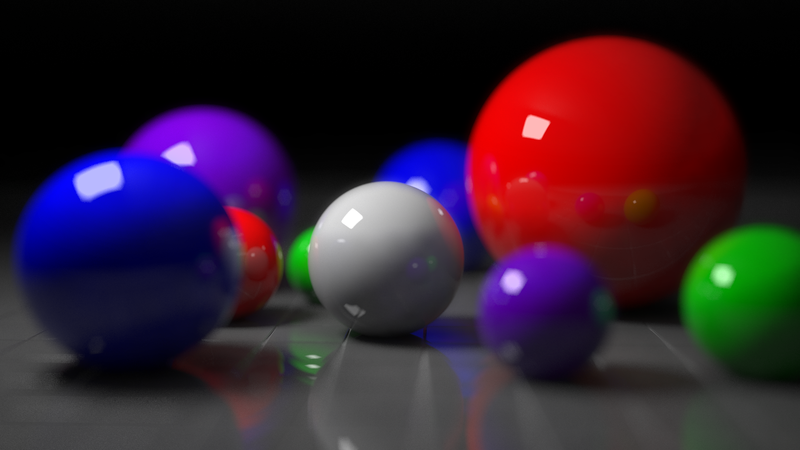
\includegraphics[width=\linewidth]{raytracing_example.png}
      \caption{Some rays have been traced}
    \end{figure}
  \end{columns}
\end{frame}

\section{Introduction}

\begin{frame}{Introduction}
  \begin{columns}
    \column{0.5\textwidth}
    \begin{itemize}
    \item Reproducing the macroscopic behavior of light is one of the fundamental problem domains in computer graphics.
    \item Simplifying assumptions are necessary to make computation tractable.
    \item Raytracing seeks to simulate light by modeling photons as particles which propagate along straight lines.
    \item Thus, we are only concerned with what happens when light ``bounces''.
    \end{itemize}

    \column{0.5\textwidth}
    \begin{figure}[H]
      \centering
      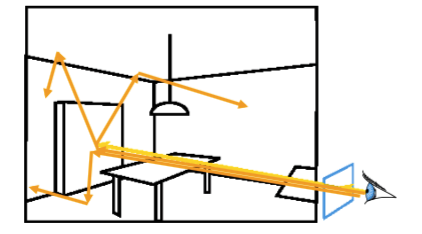
\includegraphics[width=\linewidth,keepaspectratio]{intro.png}
      \caption{Monte Carlo ray tracing}
    \end{figure}
  \end{columns}
\end{frame}

\section{Theory}


\begin{frame}{Raytracing direction}
  Raytracing can be formulated as two symmetric notions:\\[2em]
  \begin{columns}
    \column{0.5\textwidth}
    \begin{figure}[H]
      \centering
      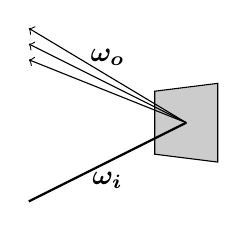
\begin{tikzpicture}
        \filldraw[color = gray!40, draw=black] (-1.4,-0.4) -- (-0.6,-0.5) -- (-0.6,0.5) -- (-1.4, 0.4) -- cycle;
        \draw[thick] (-1,0) -- (-3,-1) node[midway, below] {\(\bm{\omega_i}\)};
        \draw[->] (-1,0)  --(-3,1.2) node[midway, above] {\(\bm{\omega_o}\)};
        \draw[->] (-1,0)  --(-3,1);
        \draw[->] (-1,0)  --(-3,0.8);
      \end{tikzpicture}
      \caption{\textbf{Forward path tracing}, i.e. trace ``light rays'' from lights to eye.}
    \end{figure}

    \column{0.5\textwidth}
    \begin{figure}[H]
      \centering
      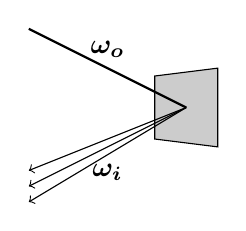
\begin{tikzpicture}
        \filldraw[color = gray!40, draw=black] (-1.4,-0.4) -- (-0.6,-0.5) -- (-0.6,0.5) -- (-1.4, 0.4) -- cycle;
        \draw[->] (-1,0) -- (-3,-0.8);
        \draw[->] (-1,0) -- (-3,-1);
        \draw[->] (-1,0) -- (-3,-1.2) node[midway, below] {\(\bm{\omega_i}\)};
        \draw[thick] (-1,0)  --(-3,1) node[midway, above] {\(\bm{\omega_o}\)};
      \end{tikzpicture}
      \caption{\textbf{Backward path tracing}, i.e. trace ``eye rays'' from eye to lights.}
    \end{figure}
  \end{columns}
  Fortunately, due to Helmholtz Reciprocity, these two methods are equivalent!
  However, since we have one camera and (often) many lights, it's easier to do backwards path tracing.
\end{frame}

\begin{frame}{Overall Behavior}
  The overall behavior of light is described by the rendering equation\footnote{this is the backward formulation}
  \[L_{o}(\mathbf x, \bm {\omega_{o}}, \lambda) = L_{e}(\mathbf x, \bm{\omega_o}, \lambda) + \int_\Omega f_s(\mathbf x, \bm{\omega_i}, \bm{\omega_o}, \lambda)L_i(\mathbf x, \bm{\omega_i}, \lambda)\ip{\bm n, \bm{\omega_i}} \dif \bm{\omega_i}\]

  \hrulefill

  \begin{center}
    \begin{tabu}{clcl}
      \(L_{o}\)& outbound radiance & \(\bm{\omega_o}\)& outbound radiance direction\\
      \(L_{i}\)& inbound radiance & \(\bm{\omega_i}\) &inbound radiance direction\\
      \(L_{e}\)& emission radiance & \(\mathbf x\) &location in space\\
      \(f_s\) & scattering distribution & \(\lambda\)& spectral wavelength\\
      \(\bm n\)& surface normal at \(\mathbf x\) & \(\Omega\) & unit hemisphere above \(\bm n\)
    \end{tabu}
  \end{center}
\end{frame}

\begin{frame}{A Model for Individual Light Bounces}
  \begin{itemize}
  \item Light bounces stochastically.
  \item Macroscopically, this behavior is a function of the \textit{material} the light is interacting with.
  \item A material is described by its \textbf{bidirectional scattering distribution function} (BSDF), notated \(f_s\).
  \end{itemize}
\end{frame}

\begin{frame}{Bidirectional Scattering Distribution Function}
  The BSDF describes the distribution of outbound light as a function of the inbound light.
  The BSDF is ususally function of four parameters.
  \[f_s(\mathbf x, \bm{\omega_i}, \bm{\omega_o}, \lambda) = \text{probability of this outcome}\]

  \hrulefill

  \begin{center}
    \begin{tabu}{cl}
      \(\mathbf x\) & point in space at which the light hit the object\\
      \(\bm{\omega_o}\) & outbound radiance direction\\
      \(\bm{\omega_i}\) & inbound radiance direction\\
      \(\lambda\) & spectral wavelength\\
    \end{tabu}
  \end{center}
\end{frame}

% \begin{frame}{Physical Properties of the BSDF}
%   \begin{itemize}
%   \item Energy conserving
%     \[\int_\Omega f_s(\mathbf x, \bm{\omega_i}, \bm{\omega_o}, \lambda)L_i(\mathbf x, \bm{\omega_i}, \lambda)\ip{\bm n, \bm{\omega_i}} \dif \bm{\omega_i} \leq L_i(\mathbf x, \bm{\omega_i}, \lambda)\]
%   \item Helmholtz Reciprocity (follows from 2\textsuperscript{nd} Law of Thermodynamics)
%     \[f_s(\mathbf x, \bm{\omega_i}, \bm{\omega_o}, \lambda) = f_s(\mathbf x, \bm{\omega_o}, \bm{\omega_i}, \lambda)\]
%   \end{itemize}
% \end{frame}

\begin{frame}{Isotropy}
  \begin{columns}
    \column{0.5\textwidth}
    \begin{enumerate}
    \item The BSDF for most materials is invariant under rotation about the surface normal.
      This behavior is called \textbf{isotropy}.

    \item Although examples of anisotropic material exist, we will ignore them here for simplicity.
    \end{enumerate}

    \column{0.5\textwidth}
    \begin{figure}[H]
      \centering
      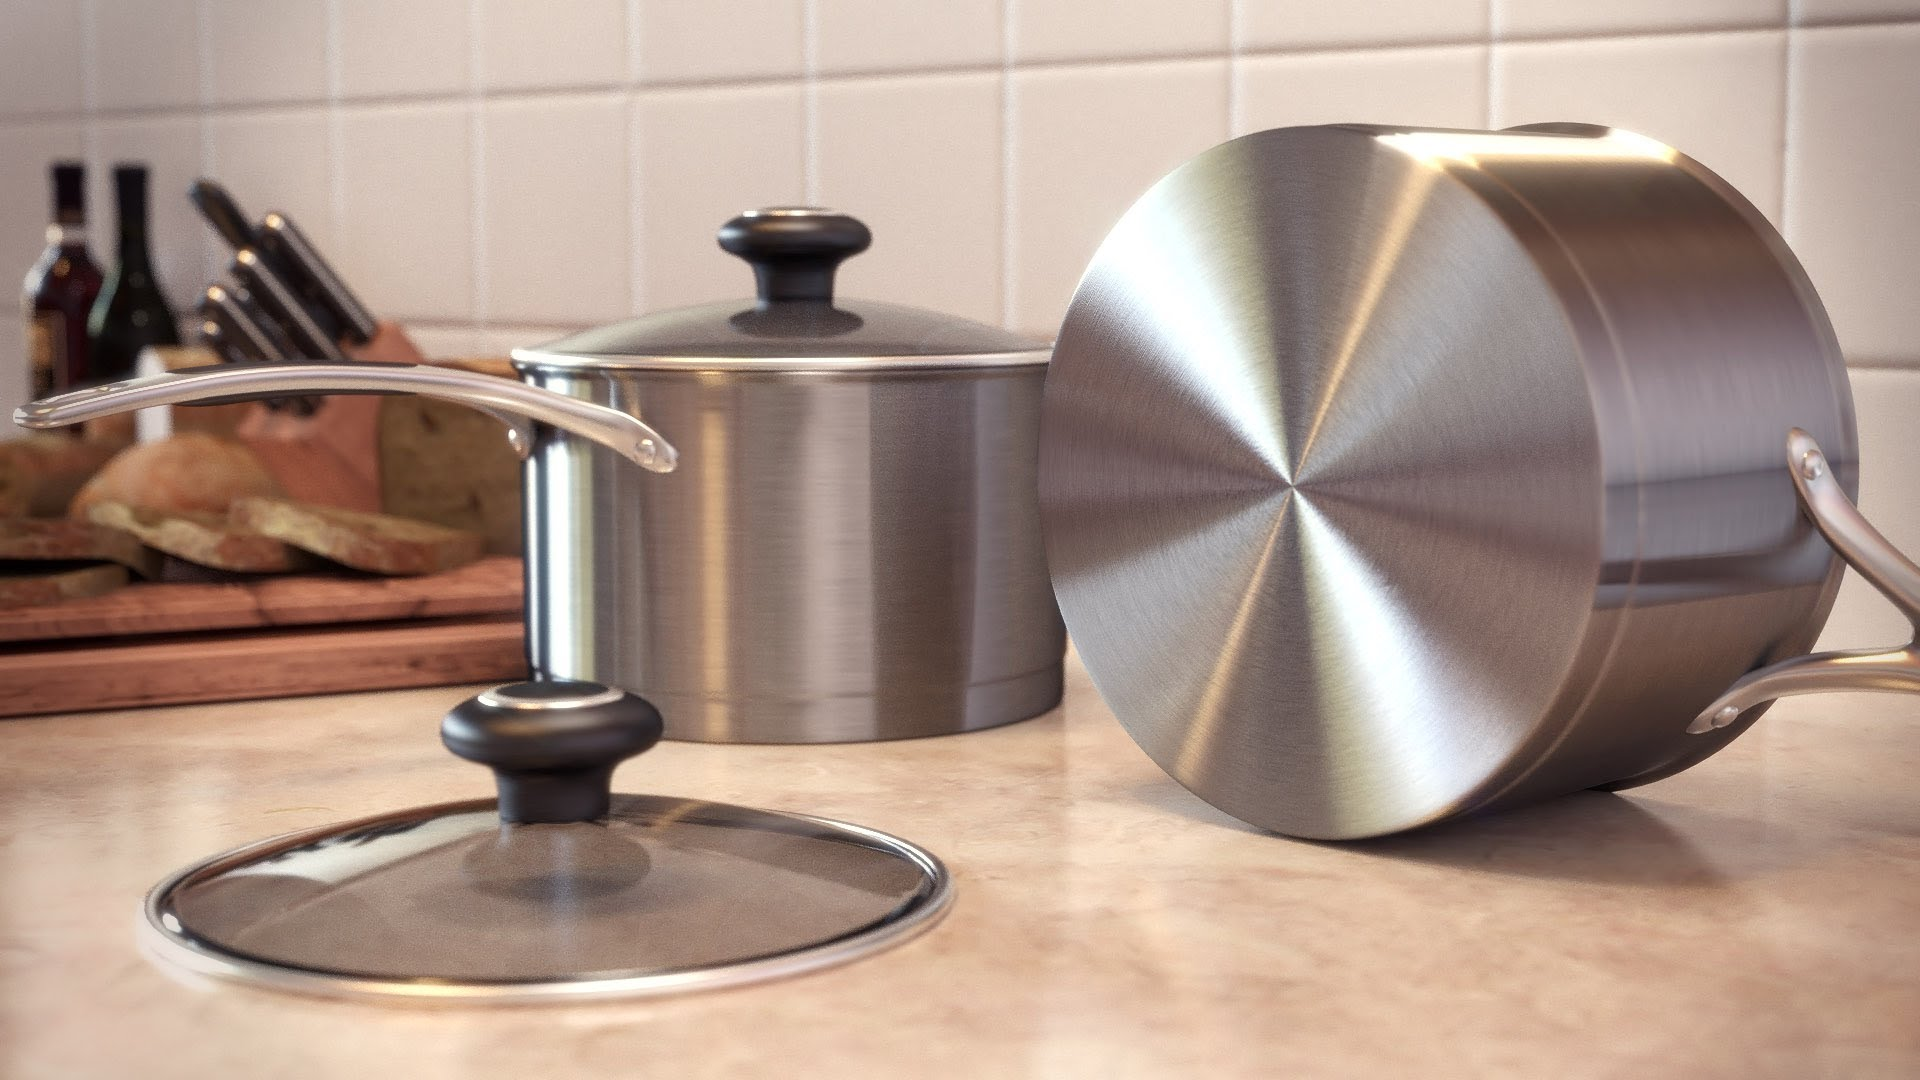
\includegraphics[width=\linewidth,keepaspectratio]{anisotropy.jpg}
      \caption{Example of Anisotropic shading.}
    \end{figure}
  \end{columns}
\end{frame}

\begin{frame}{Change of Variables}
  Since the BSDF \(f_s\) is invariant under rotation about \(\bm n\), we can rewrite \(f_s(\mathbf x, \bm{\omega_i}, \bm{\omega_o}, \lambda)\) in terms relative to \(\bm n\).
  \begin{columns}
    \column{0.5\textwidth}
    \begin{figure}[H]
      \centering
      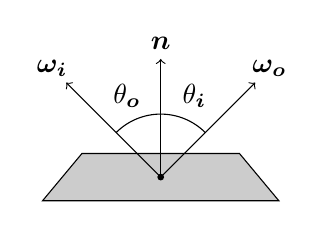
\begin{tikzpicture}
        \filldraw[color = gray!40, draw=black] (-1.5,-0.3) -- (1.5,-0.3) -- (1,0.3) -- (-1, 0.3) -- cycle;
        \draw[->] (0,0) coordinate (o) -- (-1.2,1.2) coordinate (wi) node [pos=1.15] {\(\bm{\omega_i}\)};
        \draw[->] (0,0)  --(1.2,1.2) coordinate (wo) node [pos=1.15] {\(\bm{\omega_o}\)};
        \draw[->] (0,0) -- (0, 1.5) coordinate (n) node [above] {\(\bm n\)};
        \filldraw (0,0) circle (1pt);
        \draw pic["$\theta_{\bm o}$",draw=black,angle eccentricity=1.4,angle radius=0.8cm] {angle=n--o--wi};
        \draw pic["$\theta_{\bm i}$",draw=black,angle eccentricity=1.4,angle radius=0.8cm] {angle=wo--o--n};
      \end{tikzpicture}
      \caption{Definition of \(\theta_{\bm o}\) and \(\theta_{\bm i}\).}
    \end{figure}

    \column{0.5\textwidth}
    \begin{figure}[H]
      \centering
      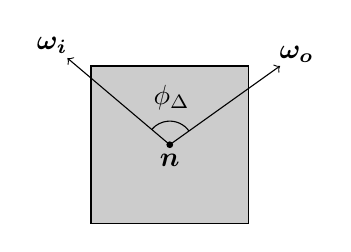
\begin{tikzpicture}
        \filldraw[color = gray!40, draw=black] (-1,-1) -- (1,-1) -- (1,1) -- (-1, 1) -- cycle;
        \draw[->] (0,0) coordinate (o) -- (-1.3,1.1) coordinate (wi) node[pos=1.15] {\(\bm{\omega_i}\)};
        \draw[->] (0,0)  --(1.4,1) coordinate (wo) node [pos=1.15] {\(\bm{\omega_o}\)};
        \node (0,0) [below] {\(\bm n\)};
        \filldraw (0,0) circle (1pt);
        \draw pic["$\phi_\Delta$",draw=black,angle eccentricity=2,angle radius=0.3cm] {angle=wo--o--wi};
      \end{tikzpicture}
      \caption{Definition of \(\phi_\Delta\).}
    \end{figure}
  \end{columns}
  \[
    \begin{aligned}
      \theta_{\bm i} &= \cos^{-1} \ip{\bm{\omega_i}, \bm n}\\
      \theta_{\bm o} &= \cos^{-1} \ip{\bm{\omega_o}, \bm n}\\
    \end{aligned}
    \qquad\phi_\Delta = \cos^{-1}\del{\frac{\ip{\bm{\omega_o} - \proj_{\bm n} \bm{\omega_o}, \bm{\omega_i} - \proj_{\bm n} \bm{\omega_i}}}{\norm{\bm{\omega_o} - \proj_{\bm n} \bm{\omega_o}} \norm{\bm{\omega_i} - \proj_{\bm n} \bm{\omega_i}}}}
  \]
\end{frame}

\begin{frame}{Integration \& Importance Sampling}
  \textbf{Recall:} Ignoring emission, we want to calculate
  \[L_{o}(\mathbf x, \bm {\omega_{o}}, \lambda) = \int_\Omega f_s(\theta_{\bm i}, \theta_{\bm o}, \phi_\Delta, \lambda)L_i(\mathbf x, \bm{\omega_i}, \lambda)\cos \theta_{\bm i} \dif \bm{\omega_i}\]
  \\[-0.5em]
  \begin{enumerate}
  \item In general, we know nothing about the distribution of \(L_i(\mathbf x, \bm{\omega_i}, \lambda, t)\).
  \item However, \(f_s(\theta_{\bm i}, \theta_{\bm o}, \phi_\Delta)\cos \theta_{\bm i}\) also has significant influence.
  \item It's still worth it to do importance sampling!
  \end{enumerate}
\end{frame}

\section{Shader Examples}

\begin{frame}{Lambert Diffuse (Introduction)}
  \begin{enumerate}
  \item ``Ideal'' diffuse: light is uniformly scattered in all directions.
  \item Simplest possible BSDF, a constant!
    \[f_s(\theta_{\bm i}, \theta_{\bm o}, \phi_\Delta) = \frac{\rho_d}{\pi}\]
  \item \(\rho_d \in \intcc{0,1}\) is the albedo, or reflectance when \( \theta_{\bm i} = \theta_{\bm o} = 0\).
  \item Present in almost all production raytracers in some form.
  \end{enumerate}
\end{frame}

\begin{frame}{Lambert Diffuse (Integral Derivation)}
  Substituting \(f_s\) into the Rendering Equation yields
  \begin{align*}
    L_{o}(\mathbf x, \bm {\omega_{o}}, \lambda)
    &= \rho_d \int_\Omega \frac{1}{\pi} L_i(\mathbf x, \bm{\omega_i}, \lambda)\cos\theta_{\bm i} \dif \bm{\omega_i}
  \end{align*}
  Now, it's important to note that this integral is with respect to solid angle.
  We can rewrite in terms of solid angle with \( \dif \omega_{\bm i} = \sin\theta_{\bm i} \dif\theta_{\bm i}\dif\phi_\Delta\) like so
  \begin{align*}
   L_{o}(\mathbf x, \bm {\omega_{o}}, \lambda) &= \rho_d \int_0^{2\pi}\int_0^{\sfrac{\pi}{2}} \frac{1}{\pi} L_i(\mathbf x, \bm{\omega_i}, \lambda)\cos\theta_{\bm i} \sin\theta_{\bm i}\dif \theta_{\bm i} \dif \phi_\Delta.
  \end{align*}
  We are interested in sampling with respect to the PDF
  \[P(\theta_{\bm i}, \phi_\Delta) = \frac{1}{\pi}\cos \theta_{\bm i}\sin \theta_{\bm i} = \frac{\sin 2\theta_{\bm i}}{2\pi}\]
\end{frame}

\begin{frame}{Lambert Diffuse (Importance Sampling Derivation)}
  \begin{enumerate}
  \item \(f_s\) doesn't depend on \(\phi_\Delta\), so we can define the PDF in terms of \(\theta_{\bm i}\)
    \[P(\theta_{\bm i}) = \int_0^{2\pi} P(\theta_{\bm i}, \phi)\dif \phi = \int_0^{2\pi} \frac{\sin 2\theta_{\bm i}}{2\pi} \dif \phi = \sin 2\theta_{\bm i}\]
  \item Integrate to find the CDF.
    \[F(\theta_{\bm i}) = \int_0^{\theta_{\bm i}} \sin 2\theta \dif \theta = \sin^2 \theta_{\bm i}\]
  \item Let \(\xi_\theta \sim \mathcal{U}(0, 1)\) and invert CDF.
    \[\xi_\theta = \sin^2 \theta_{\bm i} \implies \theta_{\bm i} = \sin^{-1}\sqrt{\xi_\theta}\]
  \item \(f_s\) is uniform with respect to \(\phi_\Delta\). When \(\xi_\phi \sim \mathcal{U}(0, 1)\), we have \(\phi_\Delta = 2\pi\xi_\phi\).
  \end{enumerate}
\end{frame}

\begin{frame}{Aside: Perfect Mirrors}
  \begin{enumerate}
  \item The direct opposite of a ideal diffuse surface is a ideal mirror.
  \item BSDF is a double Dirac delta function.
    \[f_s(\theta_{\bm i}, \theta_{\bm o}, \phi_\Delta) = \rho_s \delta(\theta_{\bm i} - \theta_{\bm o})\delta(\phi_\Delta + \pi).\]
    As before, \(\rho_s \in \intcc{0, 1}\) is the specular albedo.
  \item No sampling of the BSDF is needed. \(\bm{\omega_i}\) is uniquely determined by
    \[\bm{\omega_i} = 2\abs{\ip{\bm{\omega_o}, \bm n}}\bm n-  \bm{\omega_o}.\]
  \item Ideal mirrors aren't a good approximation for rough glossy surfaces, like unpolished metals.
  \end{enumerate}
\end{frame}

\begin{frame}{GGX Glossy (Introduction)}
  \begin{columns}
    \column{0.5\textwidth}
    \begin{enumerate}
    \item Many surfaces exhibit blurred reflection due to surface scattering.
      This is due to microscopic variation in the surface.
    \item GGX is the current state of the art for shiny surfaces.
    \item Also known as Trowbridge-Reitz Glossy.
    \end{enumerate}

    \column{0.5\textwidth}
    \begin{figure}[H]
      \centering
      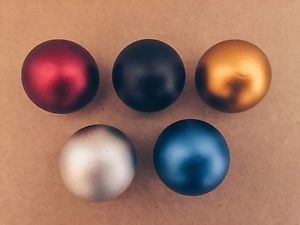
\includegraphics[width=\linewidth,keepaspectratio]{rough_glossy.jpg}
      \caption{Rough glossy spheres}
    \end{figure}
  \end{columns}
\end{frame}

\begin{frame}{GGX (Fresnel)}
  \begin{enumerate}
  \item For conductors (i.e. metals), incident light may be absorbed and converted into heat.
  \item This is described by the Fresnel term \(F(\theta_{\bm i}) = \frac{r_{\parallel}^2 + r_{\perp}^2}{2}\) which calculates the fraction of reflected light as a function of \(\theta_{\bm i}\).
  \end{enumerate}
  \[r_{\parallel}^2 = \frac{\del{\eta^2 + \kappa^2}\cos^2 \theta_{\bm i} - 2\eta \cos \theta_{\bm i} + 1}{\del{\eta^2 + \kappa^2}\cos^2 \theta_{\bm i} + 2\eta \cos \theta_{\bm i} + 1}
    \quad r_{\perp}^2 = \frac{\del{\eta^2 + \kappa^2} - 2\eta \cos \theta_{\bm i} + \cos^2 \theta_{\bm i}}{\del{\eta^2 + \kappa^2} + 2\eta \cos \theta_{\bm i} + \cos^2 \theta_{\bm i}} \]
  \\[-0.0em]
  \begin{enumerate}
    \setcounter{enumi}{2}
  \item \(\eta\) and \(\kappa\) for most metals can be found on \url{refractiveindex.info}!
  \end{enumerate}
\end{frame}

\begin{frame}{GGX Glossy (Microfacets)}
  \begin{enumerate}
  \item Blurred reflections are due to microscopic variation in the surface.
  \item The surface can be modeled as differentially tiny facets, each of which is an ideal reflector itself, called \textbf{microfacets}.
  \item The microfacet normals \(\bm m\) follow the experimentally derived distribution
  \end{enumerate}
  \[D(\bm m) = \frac{\alpha^2 \chi^+(\ip{\bm m, \bm n})}{\pi\del{\del{\alpha^2 - 1}\cos^2 \theta_{\bm m} + 1}^2}.\]

  \hrulefill

  \begin{center}
    \begin{tabu}{cl}
      \(D(\bm m)\) & PDF of the microfacet normal \(\bm m\)\\
      \(\chi^+(x)\) & equals \(1\) if \(x>0\) and \(0\) otherwise\\
      \(\theta_{\bm m}\) & is the angle between \(\bm n\) and \(\bm m\)\\
      \(\alpha > 0\) & amount of surface roughness.
    \end{tabu}
  \end{center}
\end{frame}

\begin{frame}{GGX (Smith Shadow Masking)}
  \begin{enumerate}
  \item Microfacets form a continuous microscopic surface, which casts shadows on itself.
  \item Thus it is possible for a ray \( \bm r\) to intersect with multiple microfacets.
    \begin{figure}[H]
      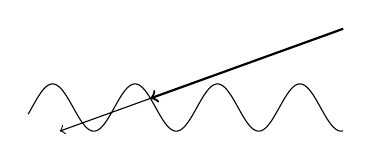
\begin{tikzpicture}[domain=1:5,samples=200]
        \draw[name path=surface] plot (\x, {0.3*sin(6*\x r)});
        \draw[name path=ray,draw=none] (5,1) -- (1.4,-0.3);
        \draw[thick,name intersections={of=ray and surface}, ->](5,1)--(intersection-3);
        \draw[name intersections={of=ray and surface}, ->](intersection-3)--(1.4,-0.3);
      \end{tikzpicture}
      \caption{A ray intersecting with a micro surface multiple times.}
    \end{figure}
    
  \item To avoid double-counting, we must employ a corrective term \(G\).

    The Smith shadow masking function approximates \(G\) as the separable product two monodirectional masking terms
    \begin{align*}
      G(\bm{\omega_i}, \bm{\omega_o}, \bm m) &= G_1(\bm{\omega_i}, \bm m)G_1(\bm{\omega_o}, \bm m)\\
      G_1(\bm v, \bm m) &= \chi^2\del{\frac{\ip{\bm v, \bm m}}{\ip{\bm v, \bm n}}} \frac{2}{1 + \sqrt{1 + \alpha^2 \tan^2{\theta_{\bm v}}}}
    \end{align*}
  \end{enumerate}
\end{frame}

\begin{frame}{GGX (Putting the Pieces Together)}
  \begin{enumerate}
  \item Given \(\bm{\omega_{i}}\) and \(\bm{\omega_{o}}\), we find the mirror microfacet unit normal to be
    \[\bm m = \frac{\bm{\omega_i} + \bm{\omega_o}}{\norm{\bm{\omega_i} + \bm{\omega_o}}}\]
  \item Thus, we can assemble the terms of the BSDF like so
    \[f_s(\theta_{\bm i}, \theta_{\bm o}, \phi_\Delta) = \rho_sF(\theta_{\bm i})D\del{\frac{\bm{\omega_i} + \bm{\omega_o}}{\norm{\bm{\omega_i} + \bm{\omega_o}}}}G\del{\bm{\omega_i}, \bm{\omega_o}, \frac{\bm{\omega_i} + \bm{\omega_o}}{\norm{\bm{\omega_i} + \bm{\omega_o}}}}\]
  \end{enumerate}
\end{frame}

\begin{frame}{GGX (Importance Sampling Introduction)}
  \begin{enumerate}
  \item Importance sampling is especially suitable for glossy surfaces, as the distribution of inbound light is highly nonuniform.
  \item In the limit as \(\alpha \to 0\) the distribution collapses towards a double Dirac delta!
  \item To simplify our calculations, we assume that \(D\) is the main contributor to the shape of the BSDF.
  \item This allows us to sample in terms of the microfacet normal \(\bm m\).
  \end{enumerate}
\end{frame}

\begin{frame}{GGX (Microfacet Importance Sampling Derivation 1)}
  \begin{enumerate}
  \item Substituting this into the rendering equation, and solving for \(\omega_i\) in terms of \(\bm m\) yields
  \end{enumerate}
  \[L_{o}(\mathbf x, \bm {\omega_{o}}, \lambda) = \int_0^{2\pi}\int_0^{\sfrac{\pi}{2}} \frac{\alpha^2 \cos\theta_{\bm m} \sin\theta_{\bm m} L_i(\mathbf x, 2\abs{\ip{\bm{\omega_o}, \bm n}}\bm n-  \bm{\omega_o}, \lambda)}{\pi\del{\del{\alpha^2 - 1}\cos^2 \theta_{\bm m} + 1}^2} \dif\theta_{\bm m}\dif\phi_\Delta \]
  \\[0em]
  \begin{enumerate}
    \setcounter{enumi}{1}
  \item Accordingly, we wish to sample the PDF
    \[P_{\bm m}(\theta_{\bm m}, \phi_\Delta) = \frac{\alpha^2 \cos\theta_{\bm m} \sin\theta_{\bm m}}{\pi\del{\del{\alpha^2 - 1}\cos^2 \theta_{\bm m} + 1}^2}\]
  \end{enumerate}
\end{frame}

\begin{frame}{GGX (Microfacet Importance Sampling Derivation 2)}
  \begin{enumerate}
  \item \(f_s\) doesn't depend on \(\phi_\Delta\), so we can define the PDF in terms of \(\theta_{\bm m}\)
  \end{enumerate}
  \[P_{\bm m}(\theta_{\bm m}) = \int_0^{2\pi}\frac{\alpha^2 \cos\theta_{\bm m} \sin\theta_{\bm m}}{\pi\del{\del{\alpha^2 - 1}\cos^2 \theta_{\bm m} + 1}^2}\dif\phi_\Delta = \frac{2\alpha^2 \cos\theta_{\bm m} \sin\theta_{\bm m}}{\del{\del{\alpha^2 - 1}\cos^2 \theta_{\bm m} + 1}^2}\]
  \begin{enumerate}
    \setcounter{enumi}{2}
  \item Integrate to find the CDF.
    \begin{align*}
      F_{\bm m}(\theta_{\bm m}) &= \int_0^{\theta_{\bm m}} \frac{2\alpha^2 \cos\theta \sin\theta}{\del{\del{\alpha^2 - 1}\cos^2 \theta + 1}^2}\dif\theta\\
      &= \frac{\alpha^2}{\alpha^2 - 1}  \del{\frac{1}{\del{\alpha^2 - 1}\cos^2\theta_{\bm m} + 1} - \frac{1}{\alpha^2}}
    \end{align*}
  \end{enumerate}
\end{frame}

\begin{frame}{GGX (Microfacet Importance Sampling Derivation 3)}
  \begin{enumerate}
    \setcounter{enumi}{3}
  \item Let \(\xi_\theta \sim \mathcal{U}(0, 1)\) and invert CDF.
    \begin{align*}
      \xi_\theta &= \frac{\alpha^2}{\alpha^2 - 1}  \del{\frac{1}{\del{\alpha^2 - 1}\cos^2\theta_{\bm m} + 1} - \frac{1}{\alpha^2}}\\
      \theta_{\bm m}&= \cos^{-1}\del{\frac{1- \xi_\theta}{\del{\xi_\theta\del{\alpha^2 - 1} + 1}}}
    \end{align*}
  \item \(f_s\) is uniform with respect to \(\phi_\Delta\). When \(\xi_\phi \sim \mathcal{U}(0, 1)\), we have \(\phi_\Delta = 2\pi\xi_\phi\).
  \item We are sampling \(\bm m\), but we need the PDF in terms of \(\bm{\omega_i}\) and \(\bm{\omega_o}\).
    To calculate the PDF, we must use the Jacobian of the transform
    \begin{align*}
      P(\omega_{\bm i}) &= P_{\bm m}\del{\frac{\bm{\omega_i} + \bm{\omega_o}}{\norm{\bm{\omega_i} + \bm{\omega_o}}} } \norm{\dpd{\bm m}{\bm{\omega_o}}}\\
                        &= \frac{1}{4\abs{\ip{\bm{\omega_i}, \bm n}\ip{\bm{\omega_o}, \bm n}}}P_{\bm m}\del{\frac{\bm{\omega_i} + \bm{\omega_o}}{\norm{\bm{\omega_i} + \bm{\omega_o}}}}
    \end{align*}
  \end{enumerate}
\end{frame}

\section{Implementation}

\begin{frame}{GitHub Repository}
  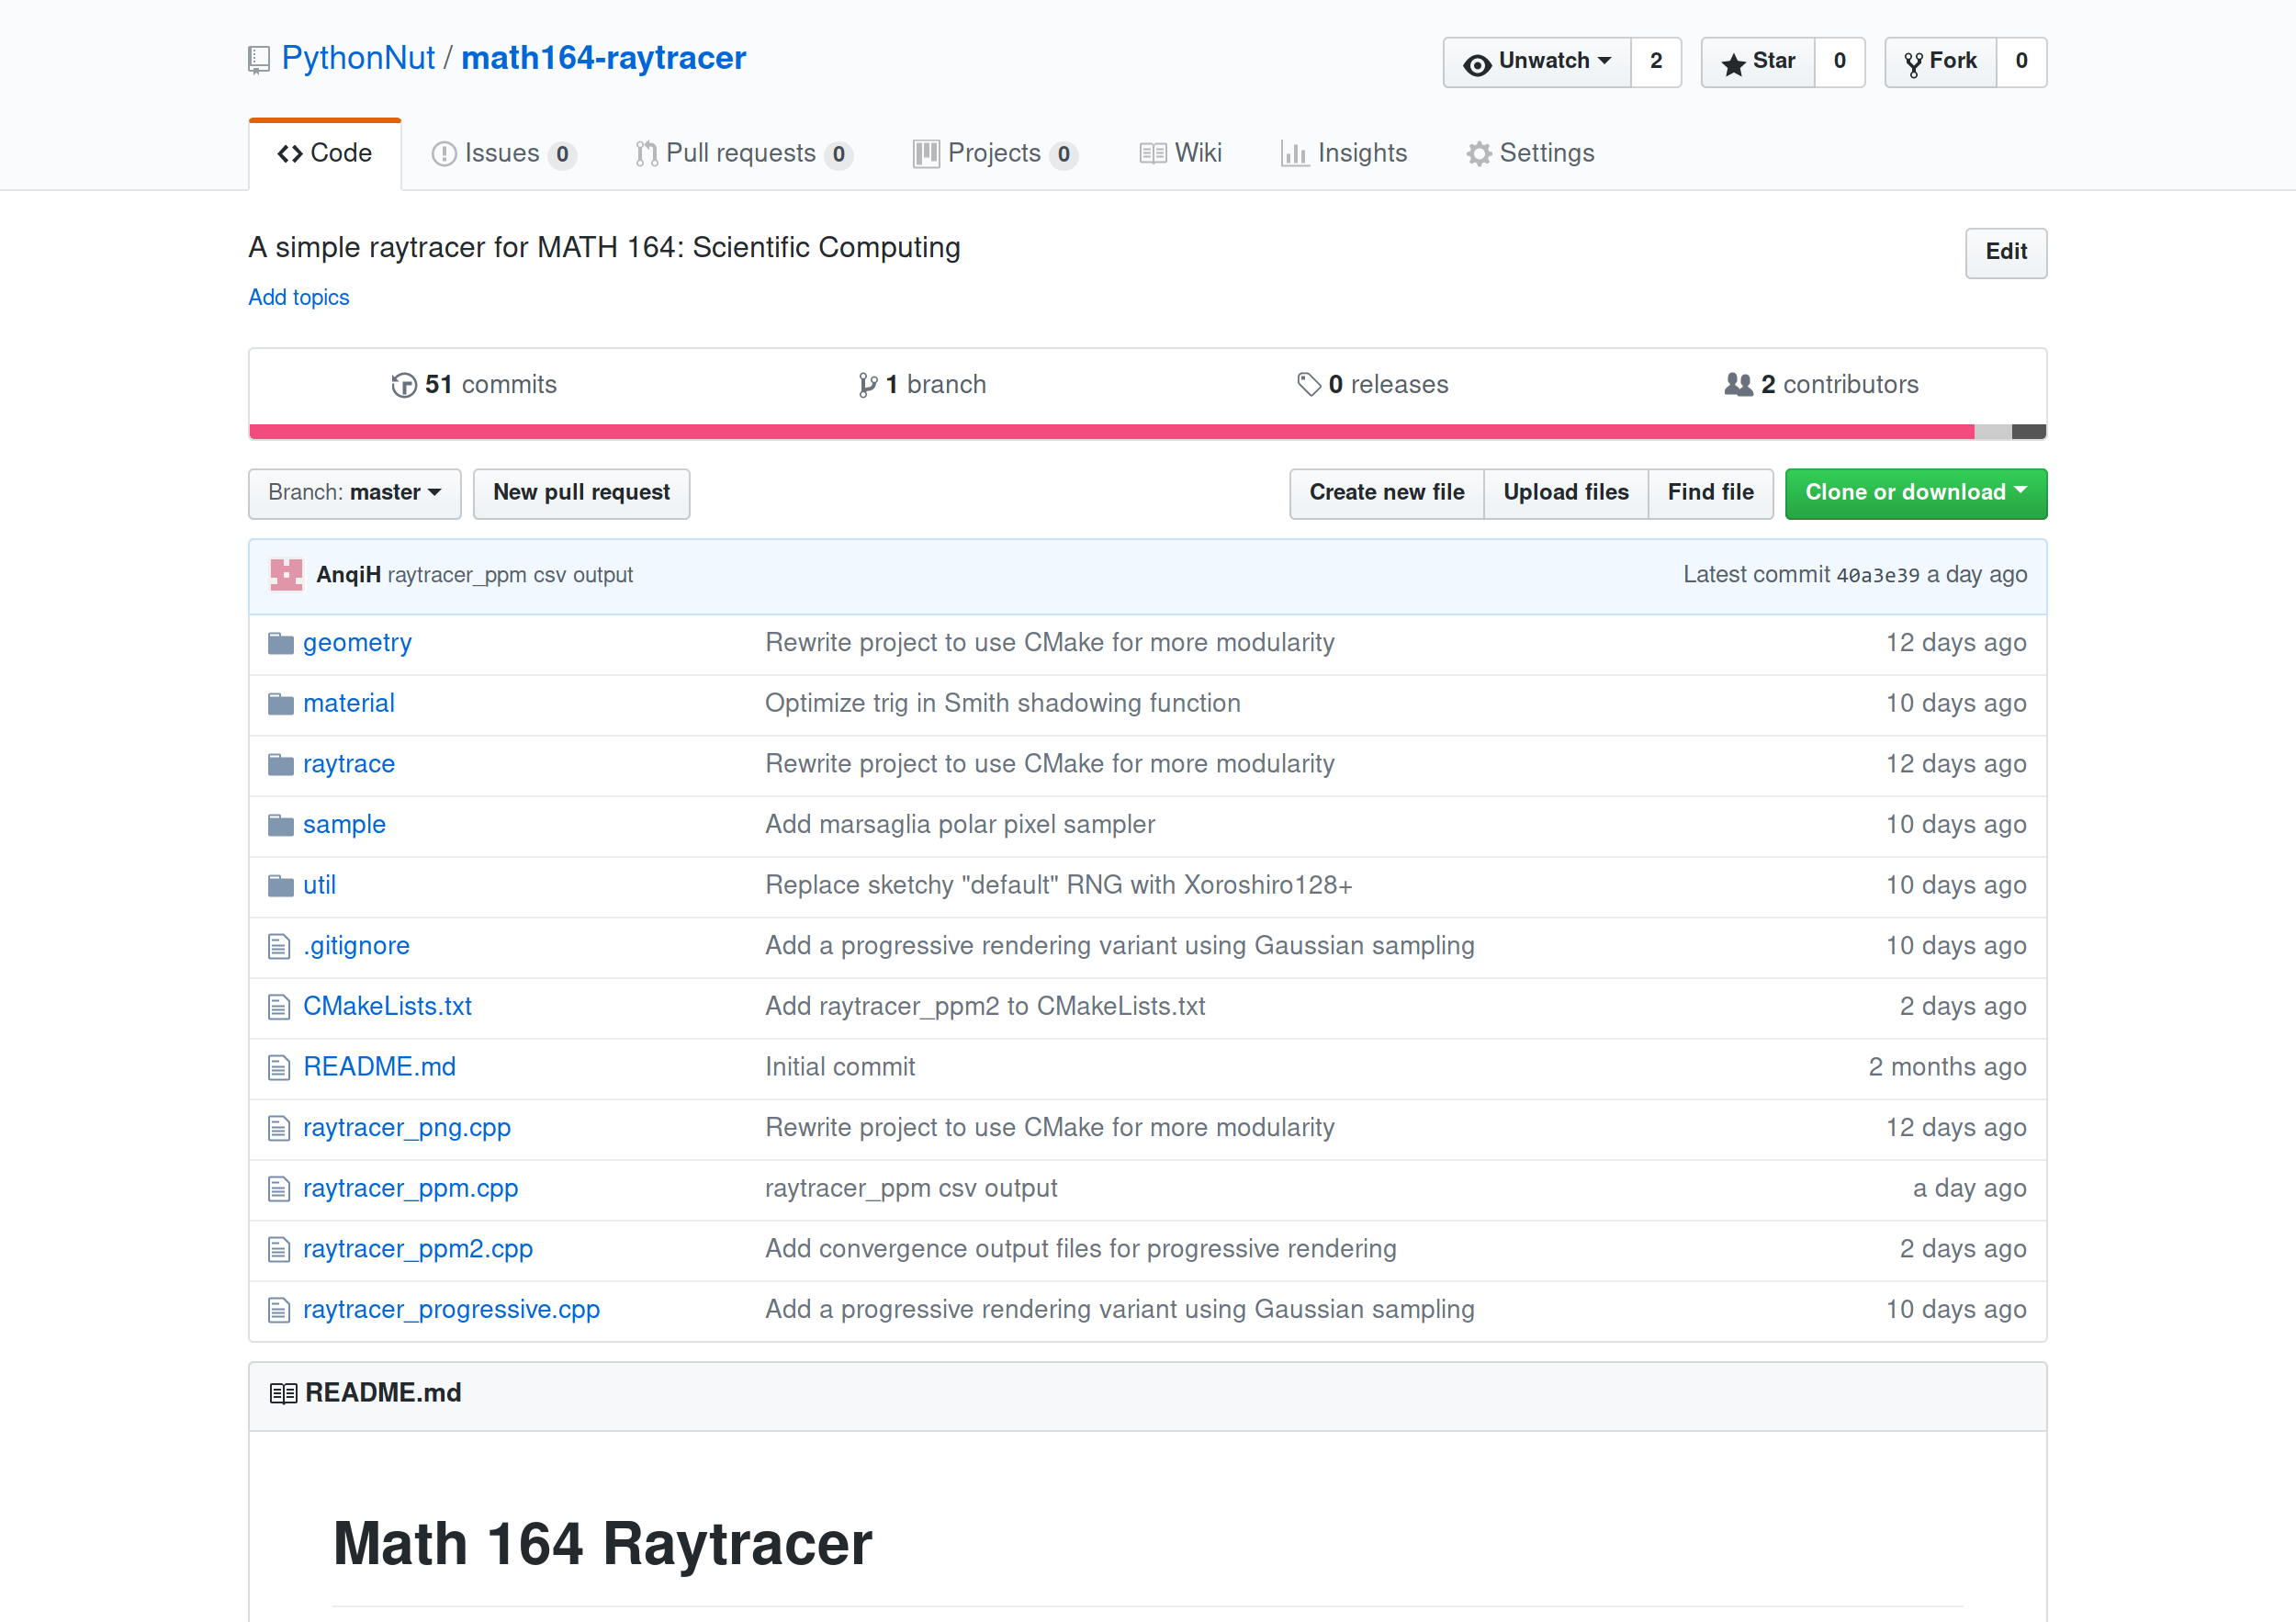
\includegraphics[width=\paperwidth, center]{github.png}
\end{frame}

\begin{frame}{Implementation Statistics}
  \begin{itemize}
  \item Written in \CC
  \item \(\approx 1,700\) lines of code
  \item Makes use of Eigen for linear algebra
  \item Multithreaded
  \item Optimized RNG (Xoroshiro128+)
  \end{itemize}
\end{frame}

\section{Results}
\begin{frame}{Rendered images}
  \begin{columns}
    \column{0.5\textwidth}
    \begin{figure}[H]
      \centering
      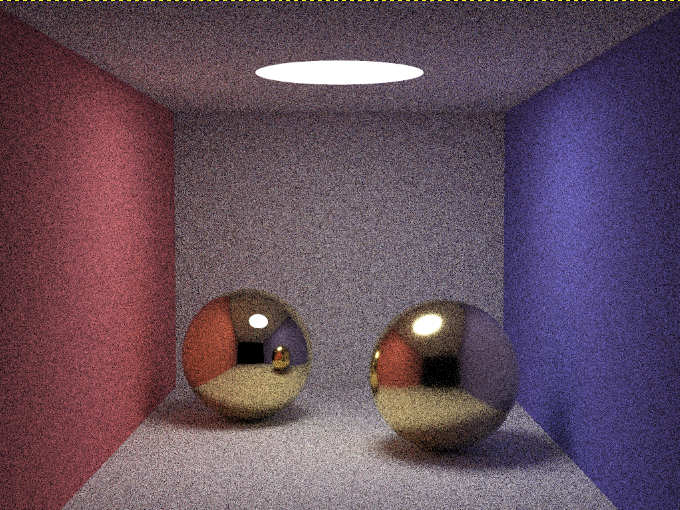
\includegraphics[width=.9\linewidth]{IS100.png}
      \caption{Importance sampling, 100 samples/pixel}
      \label{fig:sub1}
    \end{figure}

    \column{0.5\textwidth}
    \begin{figure}[H]
      \centering
      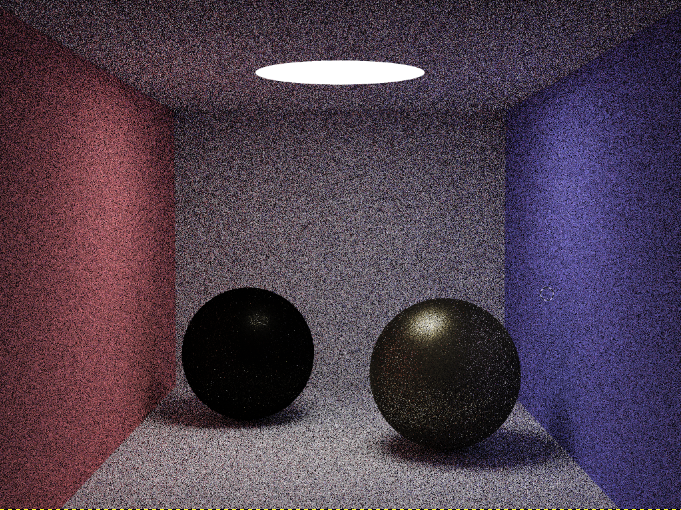
\includegraphics[width=.9\linewidth]{DS100.png}
      \caption{Uniform sampling, 100 samples/pixel}
      \label{fig:sub2}
    \end{figure}
  \end{columns}
\end{frame}

\begin{frame}
	\begin{figure}[H]
  \centering
    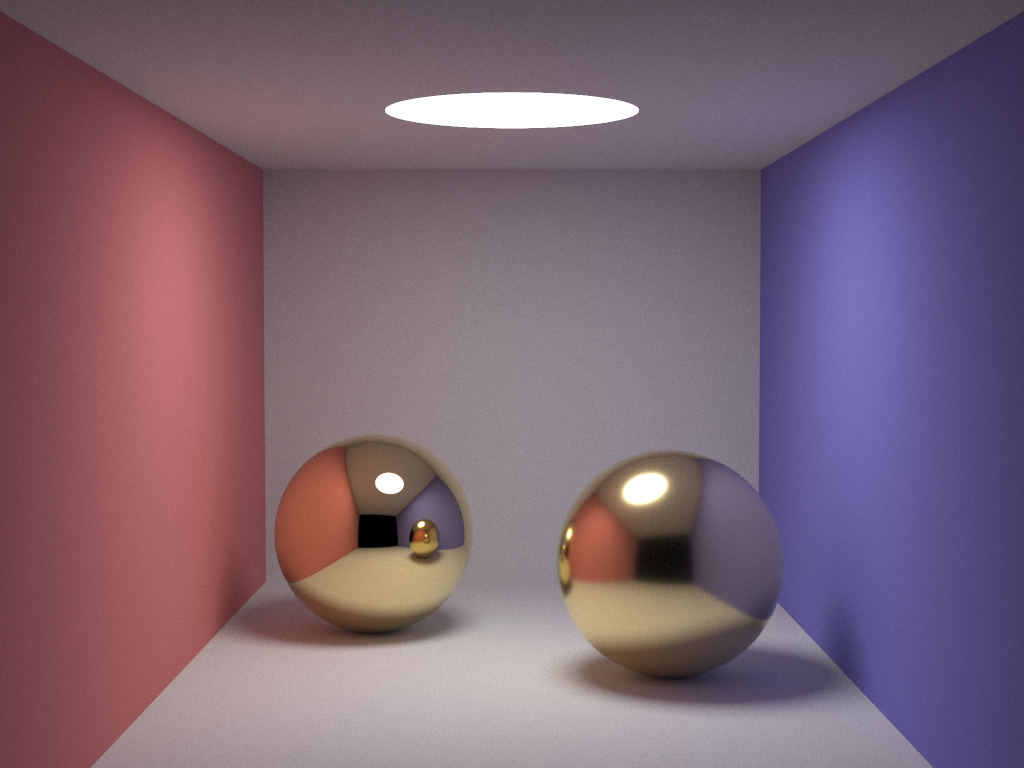
\includegraphics[width=0.9\textwidth]{convergedIS.png}
    \caption{Importance sampling, 10,000 samples/pixel}
\end{figure}
\end{frame}

\begin{frame}
	\begin{figure}[H]
  \centering
    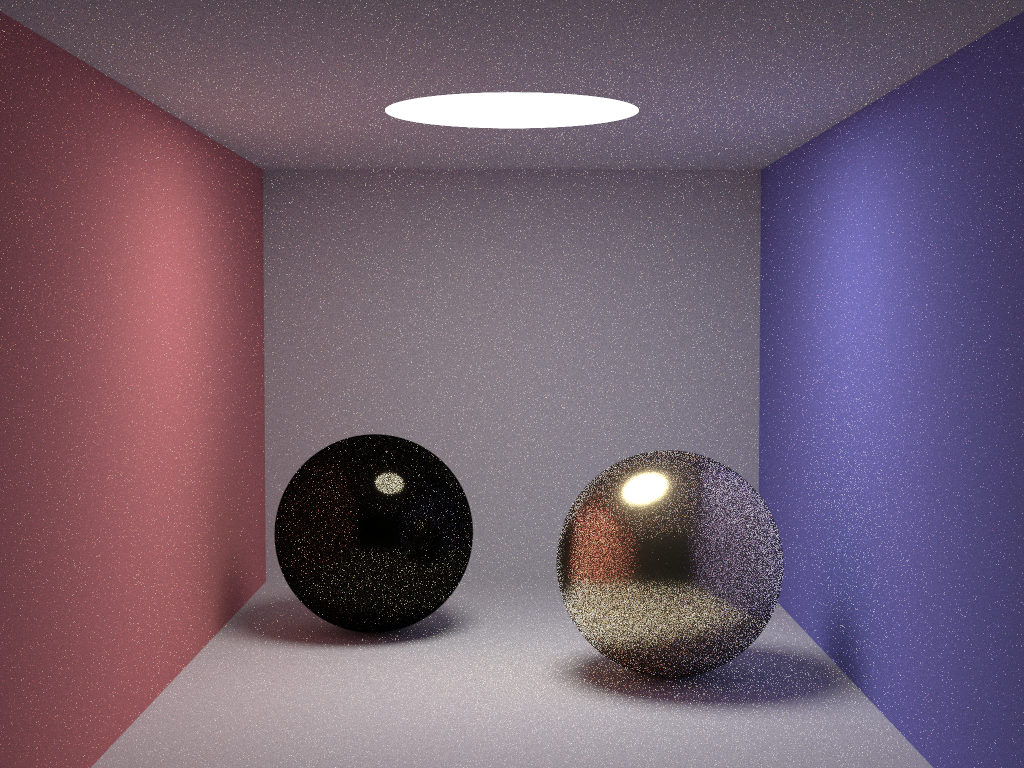
\includegraphics[width=0.9\textwidth]{10KDS.png}
    \caption{Uniform sampling, 10,000 samples/pixel}
\end{figure}
\end{frame}

\begin{frame}{Quantitatively comparing the convergence rate}
Find the absolute error between the converged image and the image rendered at a given number of samples by calculating the Mean Square Root Error of the two matrices.   
\[ \alpha = \abs{T_n - I} \]
\end{frame}

\begin{frame}
	\begin{figure}[H]
  \centering
    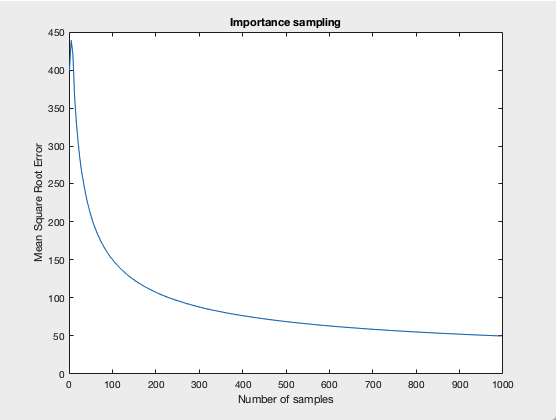
\includegraphics[width=0.9\textwidth]{importance_sampling.png}
    \caption{Importance sampling, 1000 samples/pixel}
\end{figure}
\end{frame}

\begin{frame}
	\begin{figure}[H]
  \centering
    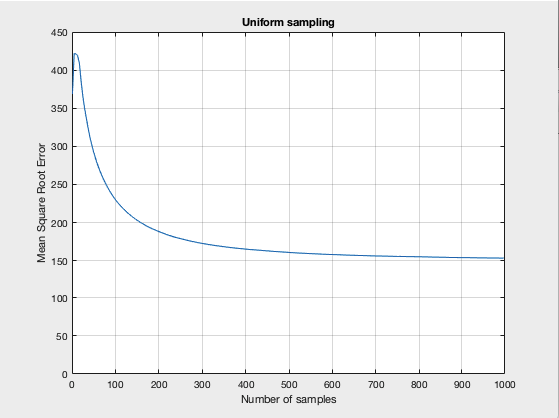
\includegraphics[width=0.9\textwidth]{direct_sampling.png}
    \caption{Uniform sampling, 1000 samples/pixel}
\end{figure}
\end{frame}

\section{Discussions}
\begin{frame}{}
\begin{itemize}
\item Quasi-Monte Carlo
\end{itemize}
\end{frame}
\end{document}
